\documentclass[12pt,a4paper]{article}
\usepackage[utf8]{inputenc}
\usepackage[T1]{fontenc}
\usepackage[spanish]{babel}
\usepackage{amsmath,amssymb}
\usepackage{graphicx}
\usepackage{booktabs}
\usepackage{geometry}
\usepackage[hidelinks]{hyperref}
\geometry{left=3cm,right=3cm,top=3cm,bottom=3cm}

\renewcommand{\contentsname}{Índice}
\renewcommand{\tablename}{Cuadro}
\renewcommand{\figurename}{Figura}

\begin{document}

% ---------------- Portada ----------------
\begin{center}
{\large Universidad Sergio Arboleda}

\vspace{1cm}
{\large Inteligencia Artificial}

\vspace{3cm}
{\LARGE\bfseries Optimización por Colonia de Hormigas}

\vspace{0.4cm}
{\Large Taller de optimización combinatoria: el Agente Viajero}

\vspace{4cm}
{\bfseries Integrantes:}

Lina Castañeda

Jorge García

Brayan Hernandez

\vspace{2cm}
{\bfseries Docente:}

Joaquin Sánchez

\vspace{4cm}
Bogotá D.C.

2026
\end{center}
\newpage

% ---------------- Índice ----------------
\tableofcontents
\newpage

% ---------------- 1 ----------------
\section{Introducción}

La optimización por colonia de hormigas (\textit{Ant Colony Optimization}, ACO)
es una metaheurística inspirada en el comportamiento de las hormigas reales para
encontrar caminos cortos entre su nido y las fuentes de alimento. Las hormigas
artificiales construyen soluciones de forma probabilística guiadas por rastros de
feromona y por información heurística del problema.

En este taller se diseñó e implementó un algoritmo ACO para resolver el problema
del Agente Viajero (\textit{Travelling Salesman Problem}, TSP). El objetivo no es
solamente encontrar tours cortos, sino medir el desempeño del algoritmo en
\textbf{tiempo} y en \textbf{memoria} para tres tamaños de instancia:
20, 2000 y 200000 ciudades, ejecutando todo en local.

La implementación se realizó en C++17 con paralelismo OpenMP y se publicó en el
repositorio \texttt{github.com/JAGR1792/ACO}.

% ---------------- 2 ----------------
\section{Descripción del problema}

Se dispone de un conjunto de $n$ ciudades con coordenadas en el plano. Se debe
encontrar el recorrido cerrado más corto que visite cada ciudad exactamente una
vez y regrese a la ciudad de origen.

Las instancias son euclidianas con puntos uniformes aleatorios en
$[0,1000]^2$, generadas con semilla fija (\texttt{--seed 42}) para que sean
reproducibles. Se evaluaron tres tamaños:

\begin{center}
\begin{tabular}{ccc}
\toprule
Instancia & Ciudades & Semilla \\
\midrule
Pequeña & 20 & 42 \\
Mediana & 2000 & 42 \\
Grande & 200000 & 42 \\
\bottomrule
\end{tabular}
\end{center}

% ---------------- 3 ----------------
\section{Punto 1. Formulación del problema}

\subsection{Variable de decisión}

Una solución se representa como un tour $T = (t_1, t_2, \dots, t_n)$, la secuencia
de ciudades en el orden de visita (notación de la clase: $T_k$ es el tour de la
hormiga $k$). El tour es cerrado: después de $t_n$ se regresa a $t_1$.

\subsection{Función objetivo}

Se minimiza la distancia total del recorrido:

\begin{equation}
\min L(T) = \sum_{i=1}^{n-1} d(t_i, t_{i+1}) + d(t_n, t_1)
\end{equation}

donde $d(a,b)$ es la distancia euclidiana entre las ciudades $a$ y $b$.

\subsection{Número de soluciones diferentes}

Fijando la ciudad inicial y sin distinguir el sentido del recorrido, el número de
tours diferentes es:

\begin{equation}
\frac{(n-1)!}{2}
\end{equation}

Cuadro 1: Tamaño del espacio de búsqueda.
\begin{center}
\begin{tabular}{cc}
\toprule
$n$ & Tours diferentes \\
\midrule
20 & $\approx 6{,}1 \times 10^{16}$ \\
2000 & del orden de $10^{5735}$ \\
200000 & intratable por enumeración \\
\bottomrule
\end{tabular}
\end{center}

Por lo tanto, la enumeración exhaustiva solo es concebible para valores muy
pequeños de $n$, lo que justifica el uso de una metaheurística como ACO.

\subsection{Cálculo manual con un ejemplo pequeño}

Con 4 ciudades $A(0,0)$, $B(3,0)$, $C(3,4)$, $D(0,4)$ existen $(4-1)!/2 = 3$
tours diferentes (fijando $A$ como inicio):

\begin{center}
\begin{tabular}{lc}
\toprule
Tour & Longitud \\
\midrule
$A$-$B$-$C$-$D$-$A$ & $3 + 4 + 3 + 4 = 14$ \\
$A$-$B$-$D$-$C$-$A$ & $3 + 5 + 3 + 5 = 16$ \\
$A$-$C$-$B$-$D$-$A$ & $5 + 4 + 5 + 4 = 18$ \\
\bottomrule
\end{tabular}
\end{center}

El óptimo es el tour $A$-$B$-$C$-$D$-$A$ con longitud 14. Este ejemplo muestra
que la función objetivo es simplemente la suma de las aristas del recorrido
cerrado.

% ---------------- 4 ----------------
\section{Punto 2. Diseño del algoritmo ACO}

\subsection{Variante y parámetros}

Se implementó la variante \textbf{MMAS} (\textit{Max-Min Ant System})
simplificada con mejora local 2-opt. Sus parámetros fueron:

Cuadro 2: Configuración del algoritmo ACO.
\begin{center}
\begin{tabular}{lcc}
\toprule
Parámetro & Símbolo & Valor \\
\midrule
Hormigas por iteración & $m$ & 20 (n=20), 25 (n=2000) \\
Iteraciones & $t_{\max}$ & 100 (n=20), 50 (n=2000) \\
Peso de feromona & $\alpha$ & 1,0 \\
Peso heurístico & $\beta$ & 2,5 \\
Evaporación & $\rho$ & 0,1 \\
Candidatos k-NN & $k$ & 8 (n=20), 25 (n=2000) \\
\bottomrule
\end{tabular}
\end{center}

\subsection{Construcción de soluciones}

Cada hormiga construye un tour paso a paso con la regla probabilística de
transición de la clase (diapositiva 15):

\begin{equation}
p_{ij}^k = \frac{\tau_{ij}^{\alpha} \, \eta_{ij}^{\beta}}
{\sum_{l \in N_i^k} \tau_{il}^{\alpha} \, \eta_{il}^{\beta}},
\qquad j \in N_i^k
\end{equation}

Esto significa, término a término: $N_i^k$ son las ciudades que la hormiga $k$
todavía no visitó estando en $i$ (su memoria tabú); $\tau_{ij}$ es la feromona,
o sea la experiencia colectiva de la colonia en esa arista; $\eta_{ij} =
1/d_{ij}$ es la heurística, o sea la conveniencia inmediata (una arista corta
tiene mayor visibilidad); $\alpha$ pesa cuánto manda la experiencia y $\beta$
cuánto manda la cercanía. El denominador normaliza para que las
probabilidades sumen 1. La elección es sesgada pero estocástica: se elige por
ruleta, así que la opción más probable no siempre gana y se conserva
diversidad (esto responde por qué no usar selección determinista).

Para no evaluar las $n$ ciudades en cada paso se usa una \textbf{lista de
candidatos}: solo se consideran las $k$ vecinas más cercanas no visitadas
(si ya se visitaron todas, se usa el resto). Esto reduce el costo por paso de
$O(n)$ a $O(k)$.

\subsection{Actualización de feromona}

Después de completar los tours, primero se evapora (diapositiva 18):

\begin{equation}
\tau_{ij} \leftarrow (1 - \rho)\,\tau_{ij}, \qquad 0 < \rho \le 1
\end{equation}

Esto significa que toda la memoria colectiva se devalúa un poco: con
$\rho = 0,1$ cada arista conserva el 90\,\% de su feromona. La evaporación es
lo que evita el estancamiento, porque las rutas que dejan de recibir refuerzo
se debilitan solas.

Luego se deposita, en proporción inversa al costo (diapositiva 19). En nuestra
variante MMAS solo la \textbf{mejor hormiga global} deposita en las aristas de
su tour:

\begin{equation}
\tau_{ij} \leftarrow \tau_{ij} + \frac{1}{L_{\text{mejor}}}
\quad \text{(solo aristas del mejor tour)}
\end{equation}

Esto significa que un tour corto aporta más feromona por arista que uno largo,
así que las buenas rutas atraen más hormigas en la siguiente iteración. Además
se recorta a $[\tau_{\min}, \tau_{\max}]$ para que ninguna arista domine para
siempre y se evite la convergencia prematura.

\subsection{Mejora local 2-opt}

Al mejor tour de cada iteración (y al mejor final) se le aplica 2-opt
\textit{first-improvement}: se prueba a reconectar pares de aristas y se acepta
el primer intercambio que acorte el tour (ventana de 40 vecinos si $n > 500$).

\subsection{Modos de ejecución}

Cuadro 3: Modos del programa.
\begin{center}
\begin{tabular}{lll}
\toprule
Modo & Uso & Descripción \\
\midrule
\texttt{full} & $n \le 5000$ & ACO denso: matriz $n \times n$ + k-NN + MMAS + 2-opt \\
\texttt{hier} & $n$ grande & Jerárquico: rejilla $\to$ ACO por celda $\to$ unión por centroides \\
\texttt{nn} & referencia & Vecino más cercano greedy (+ 2-opt si $n \le 5000$) \\
\texttt{auto} & defecto & \texttt{full} si $n \le 5000$, \texttt{hier} en otro caso \\
\bottomrule
\end{tabular}
\end{center}

El modo \texttt{hier} es necesario para 200000 ciudades: una matriz densa de
$200000^2$ valores en \texttt{float} ocuparía $\approx 149$ GB \textbf{por
matriz} (el programa lo reporta como \texttt{matrix\_mb\_est}), imposible en
local. En su lugar se particiona el plano en una rejilla de celdas de
$\approx 600$ puntos, se corre un ACO pequeño e independiente por celda y se
concatenan los subtours ordenando las celdas por centroide.

\subsection{Qué significa el modo jerárquico, paso a paso}

\texttt{hier} significa que el problema grande se parte en problemas pequeños
que sí caben en memoria, se resuelve cada uno con ACO y luego se pegan las
soluciones. Concretamente, para $n = 200000$ y
\texttt{--target-cluster 600}:

\begin{enumerate}
\item \textbf{Rejilla.} Se calcula $G = \lceil\sqrt{n/600}\rceil = 19$ y se
divide el plano en una rejilla de $19 \times 19$. Esto significa que el mapa
queda cortado en cuadros iguales, como una cuadrícula.
\item \textbf{Celdas (clusters).} Cada ciudad cae en un cuadro según sus
coordenadas. Los cuadros vacíos se descartan; en la ejecución quedaron
$361$ celdas con $\approx 550$ ciudades cada una. Esto lo muestra la línea
\texttt{[hier] n=200000 G=19 clusters=361}: $G$ es el lado de la rejilla y
\texttt{clusters} las celdas no vacías.
\item \textbf{ACO por celda.} Cada celda se resuelve como un TSP independiente
con el mismo algoritmo MMAS + 2-opt, pero en pequeño: $\approx 10$ hormigas,
$15$--$25$ iteraciones y $k = 15$ candidatos. Esto significa que cada celda
usa matrices de $\approx 600 \times 600$ ($\approx 1,4$ MB) en vez de una
matriz global de $200000 \times 200000$. Las celdas se resuelven en paralelo
con OpenMP.
\item \textbf{Orden de las celdas.} Se calcula el centroide (punto promedio) de
cada celda y se ordenan las celdas con vecino más cercano entre centroides.
Esto significa que el recorrido visita las celdas en un orden geográficamente
razonable, sin saltar de un extremo del mapa al otro.
\item \textbf{Unión.} Se concatenan los subtours en ese orden y se obtiene el
tour global de 200000 ciudades. Esto significa que las uniones entre celdas
son greedy (se pegan tal cual), por lo que se pierde optimalidad global a
cambio de hacerlo computable.
\end{enumerate}

Por eso en el CSV la fila de 200000 dice \texttt{ants=20, iters=100}: son los
valores globales del CLI, pero cada celda corre su propio ACO de
$\approx 10$ hormigas $\times$ $15$--$25$ iteraciones. Y
\texttt{--target-cluster 600} significa el tamaño de celda deseado: con un
valor menor hay más celdas (más rápido, peor calidad en las uniones); con un
valor mayor hay menos celdas (mejor calidad, más memoria y tiempo por celda).

\subsection{Complejidad: de dónde sale cada Big-O}

La complejidad se deriva contando operaciones del código (\texttt{src/aco.h},
\texttt{src/tsp.h}), con $t$ iteraciones, $m$ hormigas, $n$ ciudades y $k$
candidatos:

\textbf{Tiempo en modo \texttt{full}.} Construir el tour de una hormiga son
$n$ pasos; en cada paso se evalúan a lo sumo $k$ candidatas
($\tau^\alpha \cdot \eta^\beta$ por candidata), o sea $O(n \cdot k)$ por
hormiga. Con $m$ hormigas por iteración: $O(m \cdot n \cdot k)$ por iteración.
Con $t$ iteraciones: $O(t \cdot m \cdot n \cdot k)$. El 2-opt con ventana $w$
añade $O(n \cdot w)$ por aplicación, menor que la construcción. Sin lista de
candidatos ($k = n$) esto sería $O(t \cdot m \cdot n^2)$: por eso existe la
lista. Con los valores del experimento ($t = 50$, $m = 25$, $k = 25$), el
trabajo crece linealmente con $n$, como confirma la recta de referencia
$O(n)$ en la gráfica de escalamiento.

\textbf{Memoria en modo \texttt{full}.} Dos matrices densas de $n \times n$ en
\texttt{float} (distancias + feromona): $2 \cdot n^2 \cdot 4$ bytes, o sea
$O(n^2)$. Más el k-NN ($n \cdot k$ enteros) y los tours ($m \cdot n$ enteros),
despreciables frente a las matrices. Verificación con números: para
$n = 2000$, $2 \cdot 2000^2 \cdot 4 = 32$ MB teóricos y el programa midió 52
MB pico (el resto son hilos OpenMP y estructuras auxiliares). Para
$n = 5000$: $200$ MB teóricos, $300$ MB medidos. Para $n = 200000$:
$2 \cdot 200000^2 \cdot 4 \approx 298$ GB ($\approx 149$ GB por matriz),
imposible en local: por eso el programa se niega a usar \texttt{full} ahí. La
gráfica de memoria valida el $O(n^2)$ con su recta de referencia, mientras el
punto \texttt{hier} queda muy por debajo de ella.

\textbf{Modo \texttt{hier}.} Con $C$ celdas de $\approx c$ ciudades
($C \approx n/c$), cada celda cuesta un ACO completo pequeño
$O(t_c \cdot m_c \cdot c \cdot k)$; el total es
$C$ veces eso, o sea proporcional a $n$ (lineal) con constantes pequeñas.
Ordenar las $C$ celdas por centroide cuesta $O(C^2)$, despreciable
($C = 361$). En memoria solo vive el vector de $n$ puntos, $O(n)$, más una
celda a la vez en cada hilo, $O(c^2)$ con $c \approx 600$.

Las hormigas de cada iteración se construyen en paralelo con OpenMP (reparte
tiempo entre núcleos, no cambia el Big-O).

% ---------------- 5 ----------------
\section{Punto 3. Implementación y comandos de ejecución}

\subsection{Estructura del repositorio}

\begin{itemize}
\item \texttt{src/tsp.h}: instancia euclidiana, matriz densa, k-NN exacto.
\item \texttt{src/aco.h}: solver MMAS + 2-opt.
\item \texttt{src/main.cpp}: CLI, modos, particionado en rejilla, salida CSV.
\item \texttt{src/metrics.h}: cronómetro (\texttt{chrono}) y pico de RAM (\texttt{getrusage}).
\item \texttt{CMakeLists.txt}: compilación \texttt{Release -O3} con OpenMP.
\item \texttt{scripts/run\_benchmark.sh}: corre los 3 casos y genera \texttt{results.csv}.
\item \texttt{scripts/plot.py}: genera \texttt{img/benchmark.png}.
\end{itemize}

\subsection{Compilación}

Vía CMake (recomendada):
\begin{verbatim}
cmake -S . -B build -DCMAKE_BUILD_TYPE=Release
cmake --build build -j$(nproc)
\end{verbatim}

Vía manual, sin cmake (un solo comando):
\begin{verbatim}
g++ -O3 -std=c++17 -fopenmp src/main.cpp -o aco
\end{verbatim}

\subsection{Comandos de ejecución}

\begin{verbatim}
# 20 ciudades: ACO completo
./build/aco --n 20 --ants 20 --iters 100 --cand 8 \
  --seed 42 --mode full

# 2000 ciudades: ACO completo con 25 candidatos
./build/aco --n 2000 --ants 25 --iters 50 --cand 25 \
  --seed 42 --mode full --out results.csv

# 200000 ciudades: ACO jerárquico (celdas de ~600 puntos)
./build/aco --n 200000 --seed 42 --mode hier \
  --target-cluster 600 --out results.csv

# Benchmark completo + gráfica
bash scripts/run_benchmark.sh
python3 scripts/plot.py results.csv
\end{verbatim}

Parámetros: \texttt{--n} ciudades, \texttt{--ants} hormigas por iteración,
\texttt{--iters} iteraciones, \texttt{--cand} vecinos candidatos
(\texttt{0} = sin lista), \texttt{--seed} semilla, \texttt{--target-cluster}
tamaño de celda en modo \texttt{hier}, \texttt{--out} archivo CSV,
\texttt{--no-2opt} desactiva la mejora local.

\subsection{Evidencia de ejecución}

Figura 1: Salidas reales del programa en local.
\begin{verbatim}
n=20 mode=full ants=20 iters=100 seed=42 length=4460.31
  time_ms=142.6 peak_kb=4452
  matrix_mb_est=0.00 (solo modo full)

n=2000 mode=full ants=25 iters=50 seed=42 length=38698.88
  time_ms=1218.2 peak_kb=52028
  matrix_mb_est=15.26 (solo modo full)

[hier] n=200000 G=19 clusters=361
n=200000 mode=hier ants=20 iters=100 seed=42 length=408901.41
  time_ms=6988.3 peak_kb=74796
  matrix_mb_est=152587.89 (solo modo full)
\end{verbatim}

% ---------------- 6 ----------------
\section{Punto 4. Evaluación experimental}

\subsection{Resultados}

Máquina: Arch Linux, 12 núcleos, 14 GB RAM, \texttt{g++ 16.2.1}, OpenMP.
Semilla 42 en los tres casos.

Cuadro 4: Desempeño en tiempo y memoria.
\begin{center}
\begin{tabular}{cccccc}
\toprule
$n$ & Modo & Hormigas $\times$ iters & Longitud & Tiempo & Memoria pico \\
\midrule
20 & full (k=8) & $20 \times 100$ & 4460,31 & 0,14 s & 4,4 MB \\
2000 & full (k=25) & $25 \times 50$ & 38698,88 & 1,22 s & 52,0 MB \\
200000 & hier (361 celdas) & $10 \times 25$ por celda & 408901,41 & 6,99 s & 75,0 MB \\
\bottomrule
\end{tabular}
\end{center}

\begin{center}
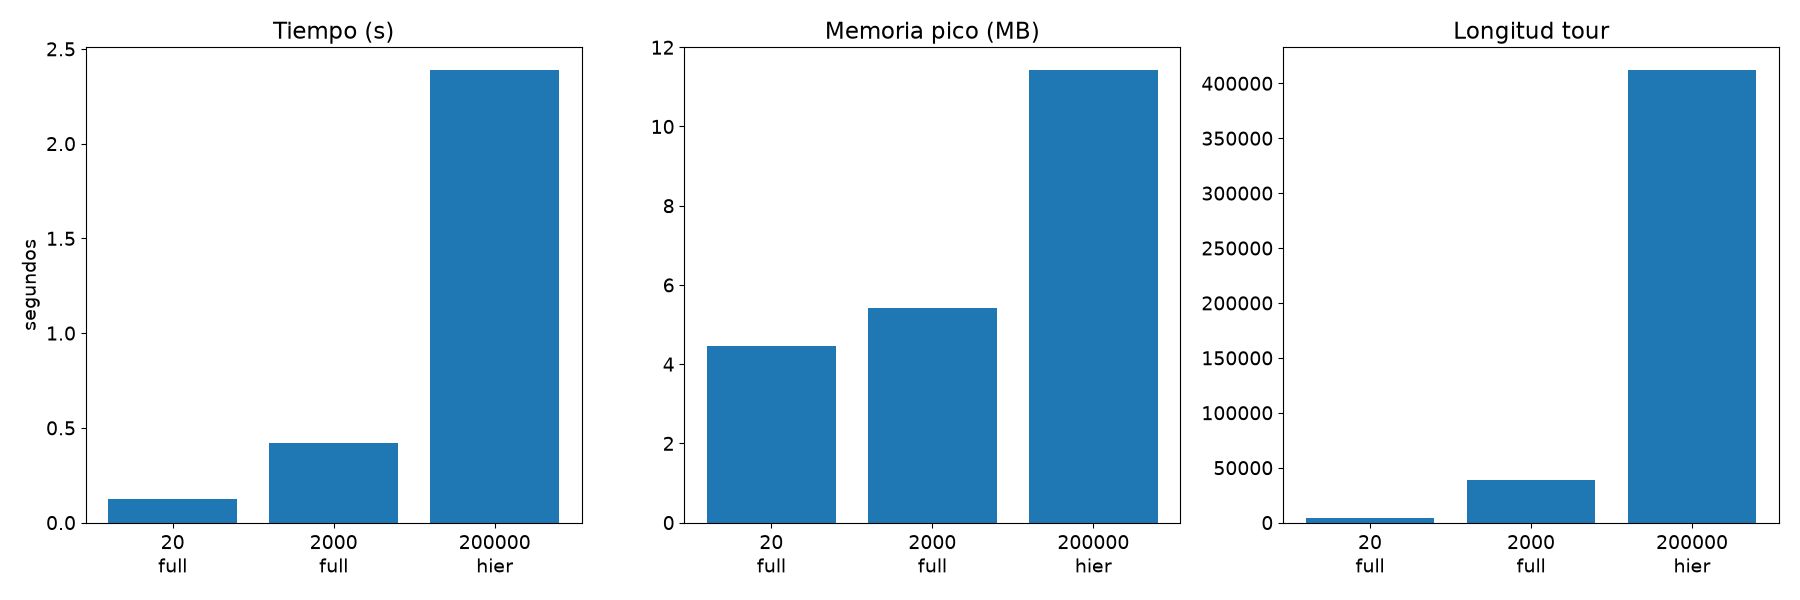
\includegraphics[width=0.95\linewidth]{../img/benchmark.png}

Figura 2: Tiempo, memoria pico y longitud del tour para los tres tamaños.
\end{center}

\subsection{Análisis de las gráficas (Figura 2)}

La Figura 2 tiene tres diagramas de barras, uno por métrica, con una barra por
tamaño (20, 2000 y 200000). Se leen así:

\textbf{Gráfica 1: Tiempo (s).} Las barras crecen de 0,14 s a 1,22 s y a 6,99
s. Esto significa que multiplicar las ciudades por 100 (de 20 a 2000) solo
multiplica el tiempo por 9: el crecimiento es subcuadrático gracias a los
candidatos. La barra de 200000 ($\approx 7$ s) es la prueba visual de que el
modo jerárquico rompe la barrera del $O(n^2)$: sin él, esa barra ni siquiera
podría existir porque el programa no cabría en memoria.

\textbf{Gráfica 2: Memoria pico (MB).} Las barras marcan 4,4 MB, 52 MB y 75
MB. Esto significa dos cosas: entre 20 y 2000 la memoria sí sigue al $O(n^2)$
de las matrices (las barras crecen fuerte), pero entre 2000 y 200000 apenas
sube de 52 a 75 MB a pesar de haber $\times 100$ ciudades. Esa segunda
transición plana es la huella del diseño jerárquico: la memoria deja de
depender de $n^2$ y pasa a depender de $n$ (el vector de puntos) más celdas de
tamaño fijo.

\textbf{Gráfica 3: Longitud del tour.} Las barras crecen (4460, 38699,
408901) simplemente porque hay más ciudades que visitar en el mismo mapa de
$1000 \times 1000$. Esto significa que esta gráfica no mide calidad del
algoritmo sino tamaño de la instancia: cada barra viene de puntos aleatorios
distintos, así que no se puede decir que una configuración sea mejor que otra
comparando estas tres barras entre sí.

\subsection{Convergencia por iteración (Figura 3)}

Para obtener esta información se agregó la opción \texttt{--trace-out}, que
guarda el mejor tour global al final de cada iteración (archivos
\texttt{trace\_20.csv} y \texttt{trace\_2000.csv}). Sacamos esta información
porque la longitud final sola no dice si las iteraciones sirvieron: la curva
muestra cuándo la colonia deja de mejorar y, por tanto, para qué sirve saber
esto es para decidir el número de iteraciones en vez de adivinarlo.

\begin{center}
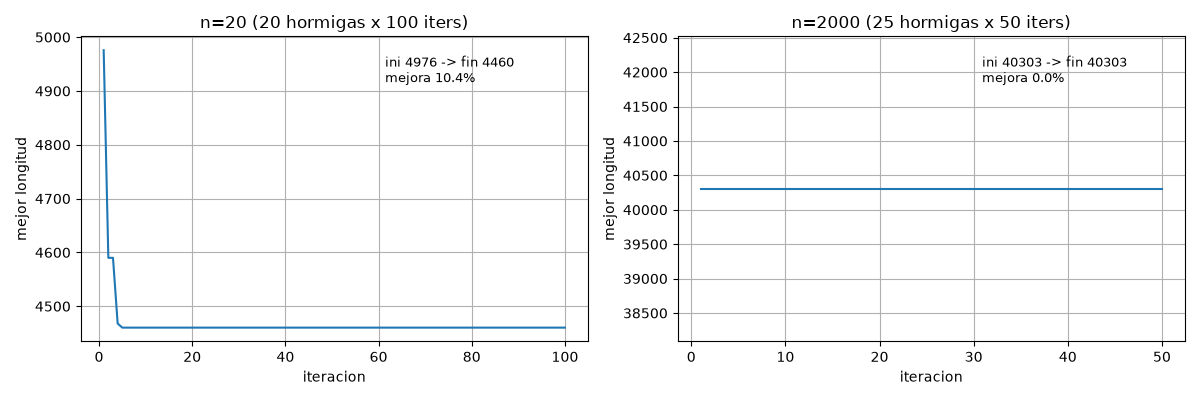
\includegraphics[width=0.95\linewidth]{../img/convergencia.png}

Figura 3: Mejor longitud global por iteración, n=20 y n=2000.
\end{center}

Con $n = 20$ la curva baja de 4975 a 4460 (10,4\,\% de mejora) y se estabiliza
alrededor de la iteración 30: esto significa que las últimas 70 iteraciones
aportaron casi nada y con $t_{\max} = 30$ bastaba. Con $n = 2000$ la curva es
plana en 40303 durante las 50 iteraciones y el salto a 38698 lo produce el
2-opt final de 2 pasadas: esto significa que, con estos parámetros, la colonia
no superó al tour greedy inicial y el trabajo lo hizo la mejora local. El
valor de saberlo es directo: para $n = 2000$ conviene invertir en más
hormigas o más 2-opt y no en más iteraciones.

\subsection{Escalamiento en tiempo y memoria (Figura 4)}

Para obtener esta información se corrió el mismo experimento
($25$ hormigas $\times$ $50$ iters, $k = 25$, semilla 42) con
$n = 100, 500, 1000, 2000, 5000$ (\texttt{scaling.csv}) más el punto
\texttt{hier} de 200000. Sacamos esta información porque un solo $n$ no
prueba un Big-O: solo una curva contra $n$, con rectas de referencia de
pendiente conocida en escala log-log, permite afirmar el orden de
crecimiento. Para qué sirve: predecir si un tamaño nuevo cabe en tiempo y
memoria antes de intentarlo.

\begin{center}
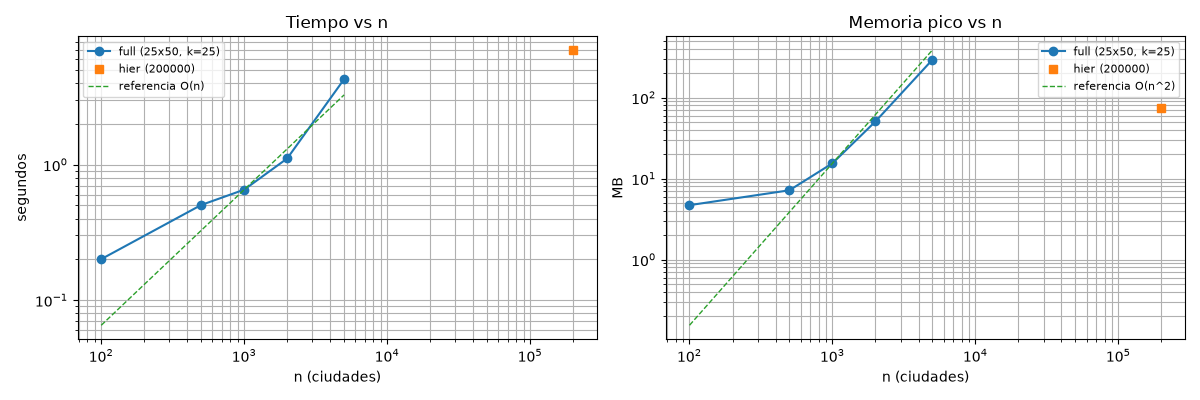
\includegraphics[width=0.95\linewidth]{../img/escalamiento.png}

Figura 4: Tiempo y memoria frente a $n$ (log-log) con referencias $O(n)$ y
$O(n^2)$, más el punto jerárquico de 200000.
\end{center}

En tiempo, los puntos \texttt{full} siguen la recta de referencia $O(n)$:
esto significa que, con $k$ fijo, duplicar las ciudades duplica el tiempo
($100 \to 5000$ ciudades: 0,2 s $\to$ 4,3 s), tal como predice
$O(t \cdot m \cdot n \cdot k)$. En memoria, los puntos \texttt{full} siguen la
referencia $O(n^2)$ ($5000$ ciudades $\Rightarrow$ $300$ MB medidos frente a
$200$ MB teóricos de matrices). El punto \texttt{hier} ($200000$ ciudades,
$7$ s, $75$ MB) queda muy por debajo de ambas rectas: es la prueba empírica
de que el particionado rompe el $O(n^2)$.

\subsection{Sensibilidad a la lista de candidatos (Figura 5)}

Para obtener esta información se varió $k \in \{5, 15, 25, 50\}$ con
$n = 2000$ y se añadió una corrida con $k = 25$ pero sin 2-opt, más una demo
pequeña ($n = 200$) con $k = 0$ (sin lista) frente a $k = 10$
(\texttt{sensibilidad.csv}). Sacamos esta información porque $k$ es el
parámetro que más afecta el costo por paso; para qué sirve: elegir $k$
justifica con datos la lista de candidatos en vez de usarla por fe.

\begin{center}
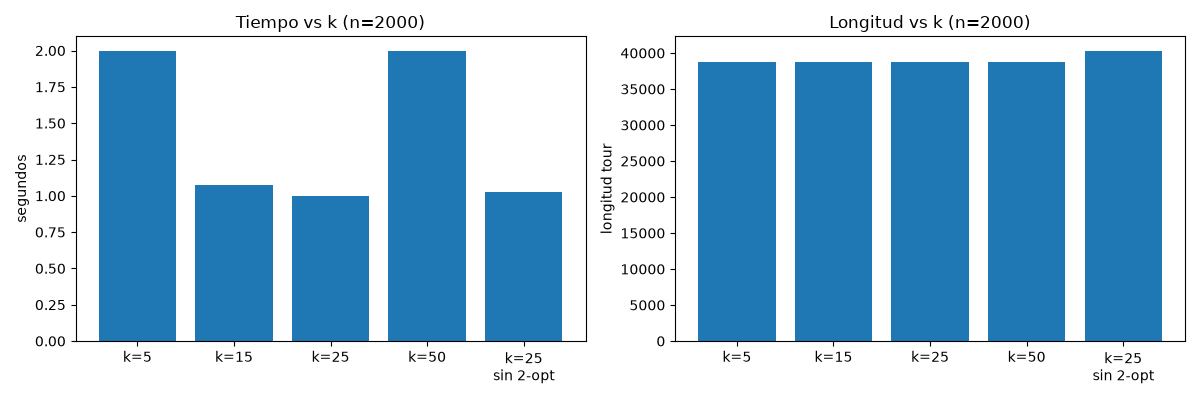
\includegraphics[width=0.95\linewidth]{../img/candidatos.png}

Figura 5: Tiempo y longitud según $k$ (n=2000), con variante sin 2-opt.
\end{center}

La longitud es idéntica (38698,88) para $k = 5, 15, 25, 50$: esto significa
que, en esta instancia, el 2-opt final corrige cualquier tour inicial y $k$
pequeño no pierde calidad. En cambio, sin 2-opt la longitud sube a 40303
(+4\,\%): esto significa que la mejora local aporta más calidad que cualquier
valor de $k$. En la demo $n = 200$, $k = 0$ tarda $139,8$ ms frente a $68,2$
ms con $k = 10$ ($\times 2$ más lento) con igual calidad: esto significa que
la lista de candidatos acelera sin degradar, y el factor crecería con $n$
porque el paso pasa de $O(n)$ a $O(k)$.

\subsection{Análisis de resultados}

\textbf{a) ¿Cómo escala el tiempo?}
De 20 a 2000 ciudades ($\times 100$ en $n$) el tiempo solo sube de 0,14 s a
1,22 s ($\times 9$), gracias a la lista de candidatos: cada paso cuesta $O(k)$
en vez de $O(n)$. El caso de 200000 se resuelve en $\approx 7$ s porque el
trabajo se divide en 361 ACOs de $\approx 550$ puntos (costo casi lineal en
$n$) más el ordenado de centroides $O(C^2)$ con $C = 361$, despreciable. Sin el
enfoque jerárquico, un ACO denso en 200000 ciudades sería intratable en tiempo
($O(t_{\max} \cdot m \cdot n^2)$ por iteración).

\textbf{b) ¿Cómo escala la memoria?}
Con $n = 20$ se usan 4,4 MB (sobrecarga base del proceso y los hilos OpenMP;
las matrices de $20 \times 20$ son insignificantes). Con $n = 2000$ se usan
52 MB: $\approx 15$ MB de distancias + $\approx 15$ MB de feromona + k-NN y
tours de 25 hormigas, coherente con el $O(n^2)$ teórico. Con $n = 200000$ se
usan solo 75 MB: nunca se construye la matriz global (que pediría $\approx 149$
GB por matriz); cada celda aloja matrices de $\approx 600 \times 600$
($\approx 1,4$ MB) y el resto es el vector de 200000 puntos. El diseño
jerárquico cambia la memoria de $O(n^2)$ a $O(n)$.

\textbf{c) ¿Qué aportan los candidatos y el 2-opt?}
Son los que más mejoran la relación calidad/tiempo: los candidatos reducen el
paso de $O(n)$ a $O(k)$ y el 2-opt corrige cruces del tour construido por las
hormigas. Desactivarlos (\texttt{--cand 0}, \texttt{--no-2opt}) empeora la
longitud, el tiempo o ambos.

\textbf{d) ¿Son comparables las longitudes entre tamaños?}
No directamente: cada $n$ usa una instancia aleatoria distinta (más ciudades
$\Rightarrow$ tour más largo). Para comparar variantes (distinto $k$, $\rho$ o
con/sin 2-opt) hay que fijar el mismo $n$ y \texttt{--seed} y mirar la columna
\texttt{length} del CSV.

\textbf{e) ¿Qué configuración se recomienda?}
Para miles de ciudades, ACO denso con $k \approx 25$ y 2-opt activado (caso
$n = 2000$: 1,2 s y 52 MB). Para cientos de miles, el esquema jerárquico con
celdas de $\approx 600$ puntos ($\approx 7$ s y 75 MB), aceptando que la unión
greedy de subtours sacrifica optimalidad global. Trabajo futuro: orientar y
coser subtours vecinos en vez de concatenar, y 2-opt entre celdas.

\subsection{Conclusión de la evaluación experimental}

\begin{enumerate}
\item El ACO clásico con matriz densa es viable hasta algunos miles de ciudades
en local (2000 $\Rightarrow$ 1,2 s, 52 MB).
\item Para 200000 ciudades el ACO puro es inviable por memoria ($\approx 149$
GB por matriz); el esquema jerárquico lo hace posible en $\approx 7$ s y 75 MB.
\item Con la misma semilla, la longitud del tour es reproducible en cualquier
máquina; tiempo y memoria solo son comparables dentro de la misma máquina.
\end{enumerate}

\section{Punto 5. Comprobación conceptual}

Respuestas a las preguntas de la clase, verificadas contra nuestra
implementación (\texttt{src/aco.h}):

\textbf{1. ¿Por qué la evaporación ayuda a evitar el estancamiento?}
Porque olvida decisiones antiguas: cada iteración multiplica toda la feromona
por $(1 - \rho)$. Las rutas que dejan de recibir refuerzo se debilitan solas y
la colonia puede abandonarlas. Sin evaporación, las primeras rutas reforzadas
dominarían indefinidamente.

\textbf{2. ¿Qué ocurre si $\alpha = 0$?}
La regla queda $p \propto \eta^{\beta}$: uso exclusivo de heurística. Cada
hormiga elige solo por cercanía, la colonia no aprende nada entre iteraciones
y el resultado equivale a un greedy estocástico repetido.

\textbf{3. ¿Qué ocurre si $\beta = 0$?}
La regla queda $p \propto \tau^{\alpha}$: uso exclusivo de feromona. Sin la
guía de la distancia, la primera ruta reforzada atrae a todas las hormigas y
la búsqueda colapsa a ella (convergencia prematura).

\textbf{4. ¿Por qué una selección determinista puede reducir la calidad final?}
Porque siempre elegiría la arista de mayor peso y todas las hormigas
construirían tours casi idénticos: se pierde diversidad y la colonia queda
atrapada en un óptimo local. Nuestra ruleta conserva aleatoriedad y por eso la
curva de $n = 20$ sigue mejorando durante 30 iteraciones en vez de
estancarse en la primera.

\textbf{5. ¿Cómo minimizar simultáneamente distancia y congestión?}
Con un costo ponderado por arista, por ejemplo
$c_{ij} = w_1 \cdot d_{ij} + w_2 \cdot g_{ij}$ (donde $g_{ij}$ es la
congestión), y heurística $\eta_{ij} = 1/c_{ij}$. En nuestro código eso es
cambiar únicamente la función de distancia: la estructura del ACO
(construcción, evaporación, depósito) se conserva y solo cambian la
heurística y el costo, como indica la clase para un cambio de dominio.

\section{Referencias}

\begin{itemize}
\item Hurbans, R. (2020). \textit{Grokking Artificial Intelligence Algorithms}.
Manning Publications. Capítulo 6: Swarm Intelligence: Ants.
\item Dorigo, M., Birattari, M., \& Stützle, T. (2006). Ant colony
optimization. \textit{IEEE Computational Intelligence Magazine}, 1(4), 28--39.
\item Dorigo, M., \& Stützle, T. (2004). \textit{Ant Colony Optimization}.
MIT Press.
\item Documento de la sesión (diapositivas 07\_IA\_2026\_2, basadas en el
capítulo 6 de Hurbans) compartido por el docente.
\item Código y datos de este taller: \texttt{github.com/JAGR1792/ACO}.
\end{itemize}

\end{document}
